
%% bare_conf.tex
%% V1.4b
%% 2015/08/26
%% by Michael Shell
%% See:
%% http://www.michaelshell.org/
%% for current contact information.
%%
%% This is a skeleton file demonstrating the use of IEEEtran.cls
%% (requires IEEEtran.cls version 1.8b or later) with an IEEE
%% conference paper.
%%
%% Support sites:
%% http://www.michaelshell.org/tex/ieeetran/
%% http://www.ctan.org/pkg/ieeetran
%% and
%% http://www.ieee.org/

%%*************************************************************************
%% Legal Notice:
%% This code is offered as-is without any warranty either expressed or
%% implied; without even the implied warranty of MERCHANTABILITY or
%% FITNESS FOR A PARTICULAR PURPOSE! 
%% User assumes all risk.
%% In no event shall the IEEE or any contributor to this code be liable for
%% any damages or losses, including, but not limited to, incidental,
%% consequential, or any other damages, resulting from the use or misuse
%% of any information contained here.
%%
%% All comments are the opinions of their respective authors and are not
%% necessarily endorsed by the IEEE.
%%
%% This work is distributed under the LaTeX Project Public License (LPPL)
%% ( http://www.latex-project.org/ ) version 1.3, and may be freely used,
%% distributed and modified. A copy of the LPPL, version 1.3, is included
%% in the base LaTeX documentation of all distributions of LaTeX released
%% 2003/12/01 or later.
%% Retain all contribution notices and credits.
%% ** Modified files should be clearly indicated as such, including  **
%% ** renaming them and changing author support contact information. **
%%*************************************************************************


% *** Authors should verify (and, if needed, correct) their LaTeX system  ***
% *** with the testflow diagnostic prior to trusting their LaTeX platform ***
% *** with production work. The IEEE's font choices and paper sizes can   ***
% *** trigger bugs that do not appear when using other class files.       ***                          ***
% The testflow support page is at:
% http://www.michaelshell.org/tex/testflow/



\documentclass[conference]{IEEEtran}
% Some Computer Society conferences also require the compsoc mode option,
% but others use the standard conference format.
%
% If IEEEtran.cls has not been installed into the LaTeX system files,
% manually specify the path to it like:
% \documentclass[conference]{../sty/IEEEtran}


\usepackage[utf8]{inputenc}
\usepackage{graphicx}
\usepackage{hyperref}

% Some very useful LaTeX packages include:
% (uncomment the ones you want to load)


% *** MISC UTILITY PACKAGES ***
%
%\usepackage{ifpdf}
% Heiko Oberdiek's ifpdf.sty is very useful if you need conditional
% compilation based on whether the output is pdf or dvi.
% usage:
% \ifpdf
%   % pdf code
% \else
%   % dvi code
% \fi
% The latest version of ifpdf.sty can be obtained from:
% http://www.ctan.org/pkg/ifpdf
% Also, note that IEEEtran.cls V1.7 and later provides a builtin
% \ifCLASSINFOpdf conditional that works the same way.
% When switching from latex to pdflatex and vice-versa, the compiler may
% have to be run twice to clear warning/error messages.






% *** CITATION PACKAGES ***
%
%\usepackage{cite}
% cite.sty was written by Donald Arseneau
% V1.6 and later of IEEEtran pre-defines the format of the cite.sty package
% \cite{} output to follow that of the IEEE. Loading the cite package will
% result in citation numbers being automatically sorted and properly
% "compressed/ranged". e.g., [1], [9], [2], [7], [5], [6] without using
% cite.sty will become [1], [2], [5]--[7], [9] using cite.sty. cite.sty's
% \cite will automatically add leading space, if needed. Use cite.sty's
% noadjust option (cite.sty V3.8 and later) if you want to turn this off
% such as if a citation ever needs to be enclosed in parenthesis.
% cite.sty is already installed on most LaTeX systems. Be sure and use
% version 5.0 (2009-03-20) and later if using hyperref.sty.
% The latest version can be obtained at:
% http://www.ctan.org/pkg/cite
% The documentation is contained in the cite.sty file itself.






% *** GRAPHICS RELATED PACKAGES ***
%
\ifCLASSINFOpdf
  % \usepackage[pdftex]{graphicx}
  % declare the path(s) where your graphic files are
  % \graphicspath{{../pdf/}{../jpeg/}}
  % and their extensions so you won't have to specify these with
  % every instance of \includegraphics
  % \DeclareGraphicsExtensions{.pdf,.jpeg,.png}
\else
  % or other class option (dvipsone, dvipdf, if not using dvips). graphicx
  % will default to the driver specified in the system graphics.cfg if no
  % driver is specified.
  % \usepackage[dvips]{graphicx}
  % declare the path(s) where your graphic files are
  % \graphicspath{{../eps/}}
  % and their extensions so you won't have to specify these with
  % every instance of \includegraphics
  % \DeclareGraphicsExtensions{.eps}
\fi
% graphicx was written by David Carlisle and Sebastian Rahtz. It is
% required if you want graphics, photos, etc. graphicx.sty is already
% installed on most LaTeX systems. The latest version and documentation
% can be obtained at: 
% http://www.ctan.org/pkg/graphicx
% Another good source of documentation is "Using Imported Graphics in
% LaTeX2e" by Keith Reckdahl which can be found at:
% http://www.ctan.org/pkg/epslatex
%
% latex, and pdflatex in dvi mode, support graphics in encapsulated
% postscript (.eps) format. pdflatex in pdf mode supports graphics
% in .pdf, .jpeg, .png and .mps (metapost) formats. Users should ensure
% that all non-photo figures use a vector format (.eps, .pdf, .mps) and
% not a bitmapped formats (.jpeg, .png). The IEEE frowns on bitmapped formats
% which can result in "jaggedy"/blurry rendering of lines and letters as
% well as large increases in file sizes.
%
% You can find documentation about the pdfTeX application at:
% http://www.tug.org/applications/pdftex





% *** MATH PACKAGES ***
%
%\usepackage{amsmath}
% A popular package from the American Mathematical Society that provides
% many useful and powerful commands for dealing with mathematics.
%
% Note that the amsmath package sets \interdisplaylinepenalty to 10000
% thus preventing page breaks from occurring within multiline equations. Use:
%\interdisplaylinepenalty=2500
% after loading amsmath to restore such page breaks as IEEEtran.cls normally
% does. amsmath.sty is already installed on most LaTeX systems. The latest
% version and documentation can be obtained at:
% http://www.ctan.org/pkg/amsmath





% *** SPECIALIZED LIST PACKAGES ***
%
%\usepackage{algorithmic}
% algorithmic.sty was written by Peter Williams and Rogerio Brito.
% This package provides an algorithmic environment fo describing algorithms.
% You can use the algorithmic environment in-text or within a figure
% environment to provide for a floating algorithm. Do NOT use the algorithm
% floating environment provided by algorithm.sty (by the same authors) or
% algorithm2e.sty (by Christophe Fiorio) as the IEEE does not use dedicated
% algorithm float types and packages that provide these will not provide
% correct IEEE style captions. The latest version and documentation of
% algorithmic.sty can be obtained at:
% http://www.ctan.org/pkg/algorithms
% Also of interest may be the (relatively newer and more customizable)
% algorithmicx.sty package by Szasz Janos:
% http://www.ctan.org/pkg/algorithmicx




% *** ALIGNMENT PACKAGES ***
%
%\usepackage{array}
% Frank Mittelbach's and David Carlisle's array.sty patches and improves
% the standard LaTeX2e array and tabular environments to provide better
% appearance and additional user controls. As the default LaTeX2e table
% generation code is lacking to the point of almost being broken with
% respect to the quality of the end results, all users are strongly
% advised to use an enhanced (at the very least that provided by array.sty)
% set of table tools. array.sty is already installed on most systems. The
% latest version and documentation can be obtained at:
% http://www.ctan.org/pkg/array


% IEEEtran contains the IEEEeqnarray family of commands that can be used to
% generate multiline equations as well as matrices, tables, etc., of high
% quality.




% *** SUBFIGURE PACKAGES ***
%\ifCLASSOPTIONcompsoc
%  \usepackage[caption=false,font=normalsize,labelfont=sf,textfont=sf]{subfig}
%\else
%  \usepackage[caption=false,font=footnotesize]{subfig}
%\fi
% subfig.sty, written by Steven Douglas Cochran, is the modern replacement
% for subfigure.sty, the latter of which is no longer maintained and is
% incompatible with some LaTeX packages including fixltx2e. However,
% subfig.sty requires and automatically loads Axel Sommerfeldt's caption.sty
% which will override IEEEtran.cls' handling of captions and this will result
% in non-IEEE style figure/table captions. To prevent this problem, be sure
% and invoke subfig.sty's "caption=false" package option (available since
% subfig.sty version 1.3, 2005/06/28) as this is will preserve IEEEtran.cls
% handling of captions.
% Note that the Computer Society format requires a larger sans serif font
% than the serif footnote size font used in traditional IEEE formatting
% and thus the need to invoke different subfig.sty package options depending
% on whether compsoc mode has been enabled.
%
% The latest version and documentation of subfig.sty can be obtained at:
% http://www.ctan.org/pkg/subfig




% *** FLOAT PACKAGES ***
%
%\usepackage{fixltx2e}
% fixltx2e, the successor to the earlier fix2col.sty, was written by
% Frank Mittelbach and David Carlisle. This package corrects a few problems
% in the LaTeX2e kernel, the most notable of which is that in current
% LaTeX2e releases, the ordering of single and double column floats is not
% guaranteed to be preserved. Thus, an unpatched LaTeX2e can allow a
% single column figure to be placed prior to an earlier double column
% figure.
% Be aware that LaTeX2e kernels dated 2015 and later have fixltx2e.sty's
% corrections already built into the system in which case a warning will
% be issued if an attempt is made to load fixltx2e.sty as it is no longer
% needed.
% The latest version and documentation can be found at:
% http://www.ctan.org/pkg/fixltx2e


%\usepackage{stfloats}
% stfloats.sty was written by Sigitas Tolusis. This package gives LaTeX2e
% the ability to do double column floats at the bottom of the page as well
% as the top. (e.g., "\begin{figure*}[!b]" is not normally possible in
% LaTeX2e). It also provides a command:
%\fnbelowfloat
% to enable the placement of footnotes below bottom floats (the standard
% LaTeX2e kernel puts them above bottom floats). This is an invasive package
% which rewrites many portions of the LaTeX2e float routines. It may not work
% with other packages that modify the LaTeX2e float routines. The latest
% version and documentation can be obtained at:
% http://www.ctan.org/pkg/stfloats
% Do not use the stfloats baselinefloat ability as the IEEE does not allow
% \baselineskip to stretch. Authors submitting work to the IEEE should note
% that the IEEE rarely uses double column equations and that authors should try
% to avoid such use. Do not be tempted to use the cuted.sty or midfloat.sty
% packages (also by Sigitas Tolusis) as the IEEE does not format its papers in
% such ways.
% Do not attempt to use stfloats with fixltx2e as they are incompatible.
% Instead, use Morten Hogholm'a dblfloatfix which combines the features
% of both fixltx2e and stfloats:
%
% \usepackage{dblfloatfix}
% The latest version can be found at:
% http://www.ctan.org/pkg/dblfloatfix




% *** PDF, URL AND HYPERLINK PACKAGES ***
%
%\usepackage{url}
% url.sty was written by Donald Arseneau. It provides better support for
% handling and breaking URLs. url.sty is already installed on most LaTeX
% systems. The latest version and documentation can be obtained at:
% http://www.ctan.org/pkg/url
% Basically, \url{my_url_here}.




% *** Do not adjust lengths that control margins, column widths, etc. ***
% *** Do not use packages that alter fonts (such as pslatex).         ***
% There should be no need to do such things with IEEEtran.cls V1.6 and later.
% (Unless specifically asked to do so by the journal or conference you plan
% to submit to, of course. )


% correct bad hyphenation here
\hyphenation{op-tical net-works semi-conduc-tor}


\begin{document}
%
% paper title
% Titles are generally capitalized except for words such as a, an, and, as,
% at, but, by, for, in, nor, of, on, or, the, to and up, which are usually
% not capitalized unless they are the first or last word of the title.
% Linebreaks \\ can be used within to get better formatting as desired.
% Do not put math or special symbols in the title.
\title{Segmentación y extracción de Tumor Cerebral:\\ una aproximación simple}


% author names and affiliations
% use a multiple column layout for up to three different
% affiliations
\author{\IEEEauthorblockN{Cristóbal Donoso}
\IEEEauthorblockA{Dpto. Ciencias de la Computación\\Facultad de Ingeniería\\
Universidad de Concepción, CHILE\\
Email: cridonoso@udec.cl}
\and
\IEEEauthorblockN{Pamela Guevara y Claudio Roman}
\IEEEauthorblockA{Dpto. Ing. Biomedica\\Facultad de Ingeniería\\
Universidad de Concepción, CHILE\\
Email: pguevara@udec.cl, clauroman@udec.cl}
}

% conference papers do not typically use \thanks and this command
% is locked out in conference mode. If really needed, such as for
% the acknowledgment of grants, issue a \IEEEoverridecommandlockouts
% after \documentclass

% for over three affiliations, or if they all won't fit within the width
% of the page, use this alternative format:
% 
%\author{\IEEEauthorblockN{Michael Shell\IEEEauthorrefmark{1},
%Homer Simpson\IEEEauthorrefmark{2},
%James Kirk\IEEEauthorrefmark{3}, 
%Montgomery Scott\IEEEauthorrefmark{3} and
%Eldon Tyrell\IEEEauthorrefmark{4}}
%\IEEEauthorblockA{\IEEEauthorrefmark{1}School of Electrical and Computer Engineering\\
%Georgia Institute of Technology,
%Atlanta, Georgia 30332--0250\\ Email: see http://www.michaelshell.org/contact.html}
%\IEEEauthorblockA{\IEEEauthorrefmark{2}Twentieth Century Fox, Springfield, USA\\
%Email: homer@thesimpsons.com}
%\IEEEauthorblockA{\IEEEauthorrefmark{3}Starfleet Academy, San Francisco, California 96678-2391\\
%Telephone: (800) 555--1212, Fax: (888) 555--1212}
%\IEEEauthorblockA{\IEEEauthorrefmark{4}Tyrell Inc., 123 Replicant Street, Los Angeles, California 90210--4321}}




% use for special paper notices
%\IEEEspecialpapernotice{(Invited Paper)}




% make the title area
\maketitle

% As a general rule, do not put math, special symbols or citations
% in the abstract

\begin{abstract}
El análisis de imágenes trae consigo la aplicación de muchas técnicas. Éstas pueden ser usadas de distintas formas y en distintas configuraciones donde, generalmente, dependen mucho del caso de estudio (manteniendo siempre una componente supervisada por un humano y otra automática). El siguiente trabajo presenta la aplicación de algunas operaciones morfológicas simples para segmentar y extraer un tumor desde una imagen tri-dimensional.\\
\end{abstract}
\begin{center}
https://github.com/cridonoso/tumor\_detection
\end{center}
% no keywords




% For peer review papers, you can put extra information on the cover
% page as needed:
% \ifCLASSOPTIONpeerreview
% \begin{center} \bfseries EDICS Category: 3-BBND \end{center}
% \fi
%
% For peerreview papers, this IEEEtran command inserts a page break and
% creates the second title. It will be ignored for other modes.
\IEEEpeerreviewmaketitle



\section{Introduction}
El procesamiento de imágenes para propósitos médicos constituye una disciplina muy amplia, encontrando así una gran cantidad de algoritmos y distintos enfoques. Actualmente, podemos tomar imágenes haciendo uso de muchas técnicas; por ejemplo, Resonancia Magnética [1]. Cada técnica entrega una cierta calidad de imagen, dependiendo del uso que se quiera dar. Sin embargo, una vez obtenida la imagen debemos procesarla para extraer información importante a partir de ésta, por ejemplo la segmentación de un tumor cerebral.\\\\ Métodos de clustering como K-means [2] son una buena alternativa a la hora de segmentar una imagen utilizando sus colores. Por otro lado, podemos utilizar algunas operaciones morfológicas como erosión y dilatación [3] para eliminar ruido o partes de la imagen que no sean de interés.\\\\En la siguiente sección se revisará el problema a resolver. Luego, se introducirá en cada una de las fases que componen la segmentación. Finalmente mostraremos los resultados obtenidos.

\section{Descripción del Problema}
El problema consiste en extraer un tumor desde una imagen 3-dimensional del cerebro. Se disponen varios casos de pacientes, por lo que cada imagen varía en tamaño, resolución y nitidez. Además, se conoce a priori la existencia del tumor. La \textit{figura 1} muestra un corte para un paciente en particular. 
\begin{figure}
\begin{center}
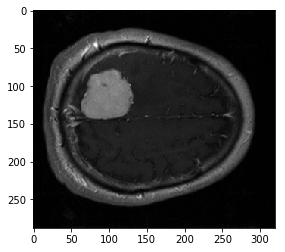
\includegraphics[scale=0.5]{img/tumor_brain.png} 
\caption{Corte transversal en escala de grises para un \textit{caso} en particular. Se distingue claramente el tumor: (case\_001\_2.nii) }
\end{center}
\end{figure}


\section{Solución Propuesta}
Podemos definir cinco fases principales. A continuación se detalla cada una de ellas
\subsection{Lectura de la Imagen y Detección del Tumor}
Lo primero es leer la imagen nifti (.nii) y llevarla a representación matricial; ésto nos permitirá poder realizar operaciones. Cabe destacar que al leer un nifti disponemos de un \textit{header} que entrega información importante respecto de la imagen. Nótese que la imagen es tridimensional y podemos hacer 33 cortes de dimensiones 288x320 (ver figura 2).\\\\
\begin{figure}
\begin{center}
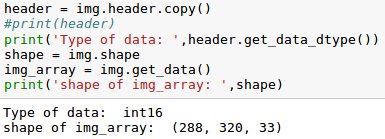
\includegraphics[scale=0.5]{img/header.png} 
\caption{Extracto de código donde se muestran las instrucciones para ver información desde el header. En particular se muestra el tipo de dato y las dimensiones de la imagen.}
\end{center}
\end{figure}
Como se mencionó anteriormente, cada imagen corresponde a casos de distintos pacientes, por lo tanto las dimensiones de la matriz pueden variar. Más aún debemos seleccionar un rango de cortes y buscar la mejor representación del tumor - para luego crear una mascara. Todo este procedimiento es empírico y realizado por un humano. La figura 3 está mostrando un buen candidato a máscara en comparación de otro corte, osea que es fácil distinguir el tumor y extrapolar la superficie de éste a lo largo de todos los cortes.
\begin{figure}
\begin{center}
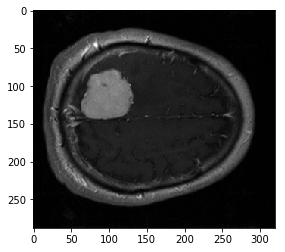
\includegraphics[scale=0.4]{img/tumor_brain.png} 
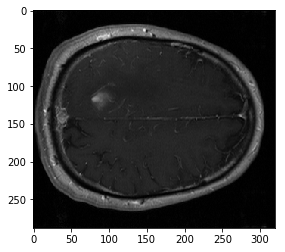
\includegraphics[scale=0.4]{img/tumor_brain_2.png} 
\end{center}
\caption{\textbf{Izquierda:} Buen representante del tumor y candidato a mascara. \textbf{Derecha:} Corte en distinto nivel de profundidad donde el tumor comienza a formarse}
\end{figure}
\subsection{Aplicación de K-means}
K-means es ampliamente usado para procesar imágenes médicas [4]. El algoritmo pertenece a la familia de técnicas no supervisadas de aprendizaje. K-means trata de particionar \textbf{n} atributos (colores) en \textbf{k} cluster mediante la busqueda de centroides. La inicialización es aleatoria, luego el método va iterando hasta definir completamente los k clusters haciendo uso de la distancia entre los datos.\\\\En este caso K-means segmenta el tumor haciendo mas fácil la extracción.\\\\Para este caso utilizamos 4 clusters. La Figura 4 muestra el siguiente paso, el cual consiste en eliminar los cluster que no coincidan con el tumor. Para ello se realizo una transformación en los valores de la matriz:
$$F_{ij} = \left\{
\begin{array}{c l}
 1 & F_{ij} \in Tumor Cluster\\
 0 & F_{ij} \not\in Tumor Cluster
\end{array}
\right.
$$ 
Donde $F_{ij}$ es el pixel en la matriz bidimensional.
\begin{figure}
\begin{center}
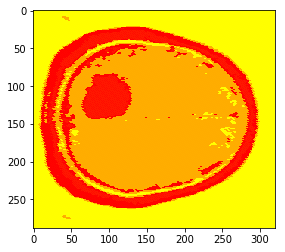
\includegraphics[scale=0.4]{img/tumor_kmeans2.png} 
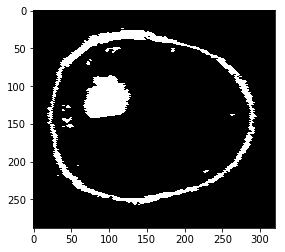
\includegraphics[scale=0.4]{img/tumor_kmeans.png} 
\end{center}
\caption{\textbf{Izquierda:} Imagen luego de aplicar k-means. \textbf{Derecha:} Imagen luego de eliminar los demás clusters.}
\end{figure}
\subsection{Erosión y Dilatación}
Luego de segmentar en función de los colores es necesario aislar el tumor. Para ello es necesario remover todo pixel que no esté dentro de los limites del tumor.\\\\La erosión y dilatación son operaciones morfológicas cuyo objetivo es borrar/agregar objetos en el imagen cuyo tamaño sea menor que un cierto kernel. Cada operación constituye la inversa de la otra, y de esta manera podemos recuperar parte del tumor que se pierde en la aplicación de la Erosión. La \textit{figura 5} muestra el proceso de erosión y dilación de la imagen.\\\\
\begin{figure}
\begin{center}
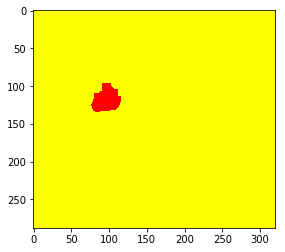
\includegraphics[scale=0.4]{img/erosion.png} 
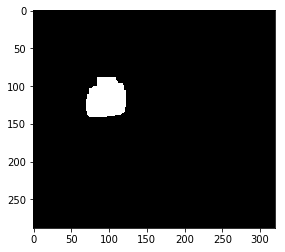
\includegraphics[scale=0.4]{img/dilation.png} 
\end{center}
\caption{\textbf{Izquierda:} Imagen luego de aplicar erosión. \textbf{Derecha:} Imagen luego de aplicar dilatación. Se utilizo un kernel cuadrado de 15x15}
\end{figure}
Una vez terminado este proceso nótese que la imagen solo preserva el tumor y los valores de cada pixel $\in {0,1}$. Por lo tanto, podemos utilizar este resultado como mascara.
\subsection{Pintando el tumor en todas las dimensiones}
Para pintar el tumor primero se considero el \textit{corte modelo}. Luego se definió un rango el cual acotaba las intensidades de gris que correspondían al tumor. La idea fué la siguiente:
\begin{center}
\textit{Recorro cada pixel en cada corte de la matriz 3-dimensional. Si el pixel tiene el color del tumor, entonces lo pinto sino lo dejo en 0.}
\end{center}
Luego aplicamos la mascara para dejar solo la porción de interés. Fue necesario además definir un rango de cortes (en este caso fue desde el [22, 29], ya que puede darse que pintemos huesos u otros tejidos dependiendo del nivel de profundidad.\\\\
\begin{figure}
\begin{center}
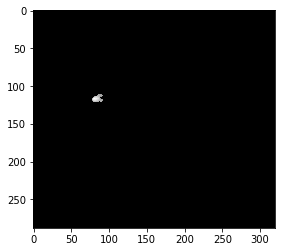
\includegraphics[scale=0.4]{img/1.png} 
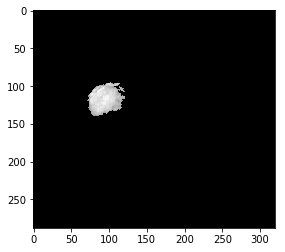
\includegraphics[scale=0.4]{img/2.png}\\
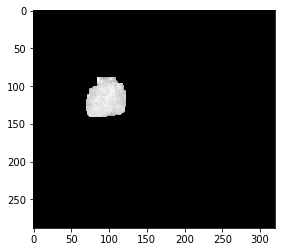
\includegraphics[scale=0.4]{img/3.png} 
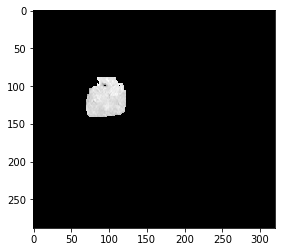
\includegraphics[scale=0.4]{img/4.png} \\
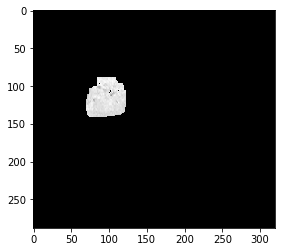
\includegraphics[scale=0.4]{img/5.png} 
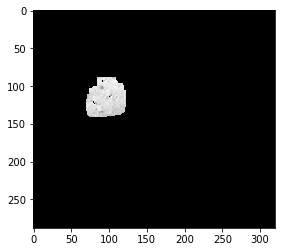
\includegraphics[scale=0.4]{img/6.png}\\
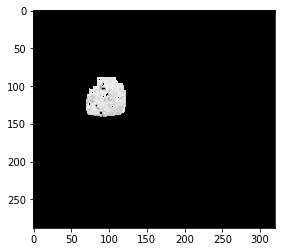
\includegraphics[scale=0.4]{img/7.png} 
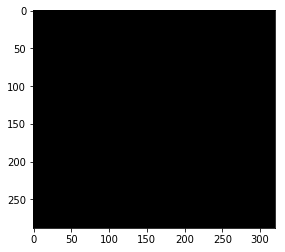
\includegraphics[scale=0.4]{img/8.png}  
\end{center}
\caption{Distintos cortes de la imagen. Se puede ver el tumor en las distintas capas de profundidad. Note que la última imagen esta vacía. Esto es porque el tumor no se distingue en ese nivel y, por lo tanto, se escapa del rango para pintar.}
\end{figure}
El resultado a lo largo de varios cortes se puede ver en la figura 6.

\subsection{Indicadores aproximados del tumor}
Finalmente, conociendo el tamaño de cada voxel (pixel en 3-dimensiones) y la cantidad de pixeles pintados podemos calcular el volumen aproximado del tumor. De igual forma, al medir la distancia máxima entre pixeles podemos calcular el diámetro aproximado del tumor. 
  
\begin{center}
\begin{tabular}{|c|c|}
\hline 
Volume & 114949.88 $mm^3$ \\ 
\hline 
Diameter & 53 $mm$ \\ 
\hline 
Mean of Voxel magnitude & 26.16 \\ 
\hline 
STD of Voxel magnitude & 176.44 \\ 
\hline 
\end{tabular} 
\end{center}

\section{Conclusión}
Se hizo uso de técnicas simples para la segmentación y extracción de un tumor. Los resultados fueron favorables pero totalmente dependientes del caso de estudio. \\\\Cada paciente tiene un anatomía distinta; por ese motivo la aproximación que se presentó en este trabajo no puede ser aplicada a una imagen distinta. En general, en el procesamiento de imágenes es necesario fijar algunos parámetros a priori (como el rango de profundidad donde aparece el tumor). La responsabilidad de esto ultimo recae únicamente en el conocimiento experto de un humano, por este motivo no se puede automatizar completamente el algoritmo.\\\\ Una solución a futuro podría consistir en entrenar un modelo de clasificación cuyo objetivo sea seleccionar los mejores parámetros dependiendo el análisis.\\\\\\\\\

\begin{thebibliography}{1}
\bibitem{IEEEhowto:kopka}
Gunther, H. (1995). NMR spectroscopy: basic principles, concepts and applications in chemistry (No. 543.42 GUN).
\bibitem{IEEEhowto:kopka}
Jain, A. K. (2010). Data clustering: 50 years beyond K-means. Pattern recognition letters, 31(8), 651-666.
\bibitem{IEEEhowto:kopka}
Haralick, R. M., Sternberg, S. R., \& Zhuang, X. (1987). Image analysis using mathematical morphology. IEEE transactions on pattern analysis and machine intelligence, (4), 532-550.
\bibitem{IEEEhowto:kopka}
Ng, H. P., Ong, S. H., Foong, K. W. C., Goh, P. S., \& Nowinski, W. L. (2006, March). Medical image segmentation using k-means clustering and improved watershed algorithm. In Image Analysis and Interpretation, 2006 IEEE Southwest Symposium on (pp. 61-65). IEEE.

\end{thebibliography}




% that's all folks
\end{document}


